\documentclass[10pt,landscape]{article}
\usepackage{multicol}
\usepackage{calc}
\usepackage{amsmath,amsthm,amsfonts,amssymb,relsize}
\usepackage{color,graphicx,overpic}
\usepackage{enumitem}
\usepackage{bm}
% \usepackage[landscape]{geometry}
\usepackage{algorithm}
\usepackage{algpseudocode}

\usepackage[cheatsheet]{preamble}
\definecolor{MyRoyalBlue}{RGB}{65,105,225} % RGB for Royal Blue
\definecolor{SubsectionGreen}{RGB}{180, 175, 80} % A soft green
% Turn off header and footer
\pagestyle{empty}
\geometry{top=.25in,left=.25in,right=.25in,bottom=.25in}


\definecolor{MyRoyalBlue}{RGB}{65,105,225} % RGB for Royal Blue
\definecolor{SubsectionGreen}{RGB}{75, 175, 80} % A soft green
\renewcommand{\CancelColor}{\color{red}} % Makes the cancel line red


% Redefine section commands to use less space
\makeatletter
\renewcommand{\section}{\@startsection{section}{1}{\z@}{3ex}{2ex}
                       {\normalfont\normalsize\bfseries\color{MyRoyalBlue}\textit}}
\renewcommand{\subsection}{\@startsection{subsection}{2}{\z@}{2ex}{0.5ex}
                          {\normalfont\small\bfseries\color{SubsectionGreen}}}
\renewcommand{\subsubsection}{\@startsection{subsubsection}{3}{0mm}%
                          {-1ex plus -.5ex minus -.2ex}%
                          {1ex plus .2ex}%
                          {\normalfont\small\bfseries}}
\makeatother

\setlist[itemize]{label={}, leftmargin=*, topsep=0pt, parsep=0.5pt, partopsep=0pt} % Remove margins from lists. 

% Don't print section numbers
\setcounter{secnumdepth}{0}

\setlength{\parindent}{0pt}
\setlength{\parskip}{0pt}

% Redefine \EndIf and \EndFunction to be empty
\algtext*{EndIf} % Removes the text "end if" on endif line
\algtext*{EndFunction} % Removes the text "end function" on end function line
\algtext*{EndFor} % Removes the text "end for" on end of forloop

\newcommand{\R}{\mathbb{R}}
\newcommand{\E}{\mathbb{E}}

\newcommand{\bb}{\mathbf{b}}
\newcommand{\bv}{\mathbf{v}}
\newcommand{\bx}{\mathbf{x}}
\newcommand{\by}{\mathbf{y}}
\newcommand{\bz}{\mathbf{z}}

\newcommand{\bA}{\mathbf{A}}
\newcommand{\bB}{\mathbf{B}}
\newcommand{\bH}{\mathbf{H}}
\newcommand{\bI}{\mathbf{I}}
\newcommand{\bJ}{\mathbf{J}}
\newcommand{\bX}{\mathbf{X}}
\newcommand{\bY}{\mathbf{Y}}
\newcommand{\bZ}{\mathbf{Z}}

\newcommand{\balpha}{\boldsymbol{\alpha}}
\newcommand{\bbeta}{\boldsymbol{\beta}}
\newcommand{\btheta}{\boldsymbol{\theta}}
\newcommand{\bmu}{\boldsymbol{\mu}}
\newcommand{\bxi}{\boldsymbol{\xi}}
\newcommand{\bSigma}{\boldsymbol{\Sigma}}
\newcommand{\bLambda}{\boldsymbol{\Lambda}}

\newcommand{\diag}{\text{diag}}
\newcommand{\tp}[1]{#1^{\prime}}
\newcommand{\inv}[1]{#1^{-1}}
\newcommand{\norm}[1]{\|#1\|}
\newcommand{\gaussian}[2]{\mathcal{N}(#1, #2)}
\newcommand{\inR}[2]{#1 \in \R^{#2}}


% \newcommand{\ruler}{\noindent\rule{\linewidth}{0.25pt}\par}
\newcommand{\ruler}{\vspace{-0.4em}\noindent\rule{\linewidth}{0.25pt}\par}



% -----------------------------------------------------------------------
\begin{document}
\raggedright%
\footnotesize
\begin{multicols*}{3}
    % multicol parameters
    % These lengths are set only within the two main columns
    % \setlength{\columnseprule}{0.1pt}
    \setlength{\premulticols}{1pt}
    \setlength{\postmulticols}{1pt}
    \setlength{\multicolsep}{1pt}
    \setlength{\columnsep}{0pt}

    \section{Math Review}
    \begin{itemize}
        \item $\bX$ and $\bY$ are \textbf{independent} iff $\Pr(\bX,\bY)=\Pr(\bX)\Pr(\bY)$
        \item $\bX$ and $\bY$ are \textbf{uncorrelated} iff $\E(\bX,\bY)=\E(\bX)\E(\bY)$
        \item \underline{Expected} value of $g(X)$: \( E[g(X)] = \int_{-\infty}^{\infty}g(x)f(x) dx\)
        \item \underline{Variance} \( \sigma^2 = E[{(X - \mu)}^2] = E[X^2] - \mu^2\)
        \item Determinant of matrix is product of its eigenvalues.
    \end{itemize}
    $
        f(\bw) = \mat{A}\va{x} + \va{x}^{\top}\mat{A} + \va{x}^{\top}\va{x} + \va{x}^{\top}\mat{A}\va{x} \Rightarrow
        \frac{df(\va{x})}{d\va{x}} = \mat{A}^{\top} + \mat{A} + 2\va{x} + \mat{A}\va{x} + \mat{A}^{\top}\va{x}
    $
    \begin{align*}
        \nabla_{\va{x}} (\va{y} \cdot \va{z}) & = (\nabla_{\va{x}} \va{y}) \va{z} + (\nabla_{\va{x}} \va{z}) \va{y} & \nabla_{\va{x}} f(\va{y}) & = (\nabla_{\va{x}} \va{y}) (\nabla_{\va{y}} f(\va{y})) \\
        \nabla_w w^T Aw                       & = (A + A^T)w                                                        & \mat{H}_{i,j}             & = \frac{\partial^2 f}{\partial x_i \partial x_j}
    \end{align*}
    \section{Perceptron (Lecture 2)}
    $f(\va{x}) = \va{w} \cdot \va{x} + \alpha = \sum_{i=1}^{d}w_i x_i + \alpha$,


    \textbf{Goal: } find $w$ s.t all constraints $y_i X_i \cdot w \ge 0$. Define a risk function and optimize it, where the loss is defined as $L(z, y_i) = -y_i z \;\text{  if } y_i z < 0, \;\text{else }0$. Therefore risk $R(w) = \sum_{i \in V}-y_i X_i \cdot w$
    \ruler%
    \textbf{Decision boundary}, a \textbf{hyperplane} in $\R^d$: $H = \{\inR{\va{x}}{d} : f(\va{x}) = 0\} = \{\inR{\va{x}}{d} : \va{w} \cdot \va{x} + \alpha = 0\}$
    \ruler%
    $\va{w}$ is the \textbf{normal} of the hyperplane,\\
    $\alpha$ is the \textbf{offset} of the hyperplane from origin,\\
    $\frac{f(\va{x})}{\norm{\va{w}}}$ is the \textbf{signed distance} from the \( \va{x} \) to hyperplane \( \mathcal{H} \).
    \ruler%
    \textbf{Perceptron algorithm},\\
    Input: $(\bx_1, y_1),\dots,(\bx_n, y_n) \in \R^{d} \times \{\pm 1\}$\\
    while some $y_i \neq \text{sign}(\va{w} \cdot \bx_i)$\\
    \-\hspace{0.5cm} pick some misclassified $(\bx_i, y_i)$\\
    \-\hspace{0.5cm} $\va{w} \leftarrow \va{w} + y_i\bx_i$
    \ruler%
    Given a \textbf{linearly separable data}, perceptron algorithm will take no more than $\frac{R^2}{\gamma^2}$ updates to \textbf{converge},
    where $R = \max_{i}{\norm{\bx_i}}$ is the radius of the data, $\gamma = \min_{i}{\frac{y_i(\va{w}\cdot\bx_i)}{\norm{\va{w}}}}$ is the margin.\\
    Also, $\frac{\va{w}\cdot\va{x}}{\norm{\va{w}}}$ is the signed distance from H to $\va{x}$ in the direction $\va{w}$.
    \ruler%
    \textbf{Gradient descent} view of perceptron, minimize margin cost function
    $J(\va{w}) = \sum_{i}{}{(-y_i(\va{w}\cdot\bx_i))}_{+}$ with $\va{w} \leftarrow \va{w} - \eta\nabla J(\va{w})$
    % --------------------------------

    \section{Support Vector Machine (Lecture 3, 4)}
    \textbf{Hard margin SVM},\\
    This method makes the margin as wide as possible.
    The signed distance from the hyperplane to $X_i$ is$\frac{f(\bx_i)}{\lVert w \rVert}$
    Hence the margin is $\min_i \frac{1}{\lVert w \rVert} |w \cdot X_i + \alpha|  \ge \frac{1}{\lVert w \rVert} \implies$
    $\min_{\va{w}} \norm{\va{w}}^2$, such that $y_i\va{w}\cdot\bx_i \geq 1 (i = 1,\dots,n)$\\
    \textbf{Soft margin SVM},\\
    $\min_{\va{w}} \norm{\va{w}}^2 + C\sum_{i = 1}^{n} \xi_i$
    \ruler%
    \textbf{Regularization and SVMs}:
    Simulated data with many features $\phi(\va{x})$;
    C controls trade-off between margin $1/\norm{\va{w}}$ and fit to data;
    Large C\@: focus on fit to data (small margin is ok). More overfitting.
    Small C\@: focus on large margin, less tendency to overfit.
    Overfitting increases with: less data, more features.
    % --------------------------------
    \section{Decision Theory (Lecture 6)}
    \textbf{Bayes Theorem:} \( \underbrace{\Pr(Y = C | X)}_{\text{Poster. Prob}} = \frac{\Pr(X | Y = C) \overbrace{\Pr(Y = C)}^{\text{Prior Prob.}}}{\Pr(X)} \)

    Assume $(\bX, \bY)$ are chosen i.i.d according to some probability distribution on $\mathcal{X}\times\mathcal{Y}$.
    \textbf{Risk} is misclassification probability:
    \begin{flalign*}
         & R(r) = \E\left[L(r(\bX), \bY)\right] = \Pr(r(\bX) \neq \bY)                                                   \\
         & =\sum_{\va{x}} \big[ L(r(\va{x}), 1)\Pr(Y = 1|x) + L(r(x), -1)\Pr(Y = -1|X = \va{x}) \big] \times \Pr(\va{x}) \\
         & = \Pr(Y = 1) \sum_x L(r(\va{x}), 1)\Pr(\va{x}|Y = 1) + \Pr(Y = -1) \sum_x L(r(\va{x}), -1)\Pr(\va{x}|Y = -1)  \\
    \end{flalign*}
    \textbf{Bayes Decision Rule} is
    $
        r^{*}(x) =
        \begin{cases}
            1,  & \text{if } L(-1, 1)\Pr(\bY=1|x) > L(1, -1)\Pr(\bY=-1|x) \\
            -1, & \text{otherwise. }
        \end{cases}
    $,\\
    and the optimal risk (Bayes risk) $R^{*} = \inf_{r}R(r)=R(r^*)$
    % --------------------------------

    \section{Generative and Discriminative Models (Lecture 6)}
    \textbf{Discriminative models}: $\Pr(\bX, \bY) = \Pr(\bX)\Pr(\bY|\bX)$.\\
    Estimate $\Pr(\bY|\bX)$, then pretend our estimate $\hat{\Pr}(\bY|\bX)$ is the actual $\Pr(\bY|\bX)$ and
    plug in bayes rule expression.
    \ruler%
    \textbf{Generative model}: $\Pr(\bX, \bY) = \Pr(\bY)\Pr(\bX|\bY)$.\\
    Estimate $\Pr(\bY)$ and $\Pr(\bX|\bY)$, then use bayes theorem to calculate $\Pr(\bY|\bX)$ and use discriminative model.
    \ruler%
    \textbf{Gaussian} class conditional densities $\Pr(\bX|Y=+1)$,$\Pr(\bX|Y=-1)$ (with the same variance), the posterior probability is \textbf{logistic}:\\
    $\Pr(Y=+1|\va{x}) = \frac{1}{1+\text{exp}(-\va{x}\cdot\va{w}-\beta_0)}$,\\
    $\va{w} = \inv{\Sigma}(\bmu_{1}-\bmu_{0})$, $\beta_0=\frac{\tp{\bmu_{0}}\inv{\Sigma}\bmu0-\bmu_{1}\inv{\Sigma}\bmu1}{2}+\log\frac{\Pr(Y=1)}{\Pr(Y=0)}$
    % --------------------------------

    \section{Multivariate Normal Distribution (Lecture 7)}
    $\inR{\va{x}}{d}: p(x) = \frac{1}{{(2\pi)}^{d/2}|\bSigma|^{1/2}}e^{(-\frac{1}{2}\tp{(\va{x}-\bmu)}\inv{\bSigma}(\va{x}-\bmu))}$
    \ruler%
    \textbf{QDA:} Class-conditional densities \( X_C \sim \gaussian{\va{\mu}_C}{\Sigma_C}\). Optimal decision rule \( r^*(x) \) for 0--1 loss: Choose class \textbf{C} that maxes \( \Pr(Y = C|X) \propto f_C(x)\pi_C \). Parameters estimated via MLE\@:

    \textbf{LDA:} Assumes equal covariance matrices across classes (\( \Sigma_C = \Sigma \)), simplifying to linear decision surfaces.
    \ruler%
    $\bSigma = \E(\bX - \bmu)\tp{(\bX - \bmu)}$\\
    Symmetric: $\bSigma_{i,j} = \bSigma_{j_i}$\\
    Non-negative diagonal entries: $\bSigma{i,i} \geq 0$\\
    Positive semidefinite: $\forall \inR{\bv}{d}, \tp{\bv}\bSigma\bv \geq 0$
    \ruler%
    Given a $d$-dimensaional Gaussian $\bX \sim \gaussian{\bmu}{\bSigma}$,\\
    matrix $\inR{\mat{A}}{m\times d}$ and vector $\inR{\bb}{m}$, define $\bY = \mat{A}\bX + \bb$.\\
    Then $\bY \sim \gaussian{\mat{A}\bmu + \bb}{\mat{A}\bSigma\mat{A}^{\top}}$
    \ruler%
    Given a $d$-dimensaional Gaussian $\bX \sim \gaussian{\bmu}{\bSigma}$,\\
    with $\bSigma$ positive definite,\\
    $\bY = \bSigma^{-\frac{1}{2}}(\bX-\bmu) \sim \gaussian{\va{0}, \bI}$
    \ruler%
    \subsection{MLE's}
    \textbf{Maximum a posterior probability}: the mode of the posterior. If uniform prior, MAP is MLE; if not
    uniform prior, MAP is Penalized MLE.
    % --------------------------------

    \begin{itemize}
        \item \textbf{Prior:} \( \hat{\pi}_C = \Pr(Y=C) = \frac{N_C}{n} \)
        \item \textbf{Mean:} \( \hat{\mu}_C = \E[\bX|Y=C] = \frac{1}{N_C} \sum\limits_{i:Y_i = C} X_i \)
        \item \textbf{Covariance:} \( \hat{\Sigma}_C = \frac{1}{N_C} \sum\limits_{i:Y_i = C} (X_i - \hat{\mu}_C)(X_i - \hat{\mu}_C)^\top \)
        \item \textbf{Pooled Cov:} \( \hat{\Sigma} = \frac{1}{n} \sum\limits_{C_k} \sum\limits_{i:Y_i = C_k} (X_i - \hat{\mu}_{C_k})(X_i - \hat{\mu}_{C_k})^\top \)
    \end{itemize}
    \section{Discriminant Analysis (Lecture 7)}
    \textbf{Discriminant Functions for LDA and QDA} for class $C$, denoted \(Q_C(\va{x})\) is:
    \[
        Q_C(\va{x}) = \ln \left( \frac{f_{\va{X}|Y=C}(\va{x}) \pi_C}{(2\pi)^{\frac{d}{2}}} \right) = -\frac{1}{2}(\va{x} - \bm{\mu}_C)^T \bm{\Sigma}_C^{-1} (\va{x} - \bm{\mu}_C) - \frac{1}{2}\ln |\bm{\Sigma}_C| + \ln \frac{\pi_C}{(2\pi)^{\frac{d}{2}}}
    \]
    Here we have, the class-conditional density \(f_{\va{X}|Y=C}(\va{x})\), prior probability \(\pi_C\), the mean vector of class \(C\), and covariance matrix \(\bm{\Sigma}_C\) of class $C$.
    \ruler%
    \textbf{Linear Decision Function between Classes C and D:}
    Compares classes by:

    \[
        Q_C(\va{x}) - Q_D(\va{x}) = (\bm{\mu}_C - \bm{\mu}_D)^T \bm{\Sigma}^{-1} \va{x} - \frac{1}{2} (\bm{\mu}_C^T \bm{\Sigma}^{-1} \bm{\mu}_C - \bm{\mu}_D^T \bm{\Sigma}^{-1} \bm{\mu}_D) + \ln \frac{\pi_C}{\pi_D}.
    \]
    This expression includes a linear term \((\bm{\mu}_C - \bm{\mu}_D)^T \bm{\Sigma}^{-1} \va{x}\), which describes how the decision boundary is formed linearly in the feature space, and a constant term that adjusts the boundary based on the means of the classes and their prior probabilities.
    \ruler%
    \textbf{Multi-class LDA:}
    The optimal class for a given feature vector \(\va{x}\) is chosen by
    \[
        \text{Choose class } C \text{ such that } Q_C(\va{x}) \text{ is maximized.}
    \]
    Effectively determining the most likely class based on the feature measurements and statistical properties of each class.

    \section{Linear Regression (Lecture 10)}
    \textbf{Objective Function:}
    The goal in linear regression is to minimize the sum of squared residuals (RSS), expressed as:
    \[
        \text{RSS}(\va{w}) = \sum_{i=1}^{n} (\va{x}_i^\top \va{w} + \alpha - y_i)^2 = \norm{\bX\va{w} - \va{y}}^2.
    \]
    Where, \(\bX \in \R^{n \times (d + 1)}\) is the \textbf{design matrix}, and \(\va{y}\) is the \textbf{response vector}.

    \textbf{Minimize via Calculus:}
    \( \nabla \text{RSS}(\va{w}) = 2\bX^\top \bX \va{w} - 2\bX^\top \va{y}. \)\\
    Setting this gradient to zero leads to the \textbf{normal equations}:
    \[
        \bX^\top\bX\va{w} = \bX^\top\va{y} \implies \va{w}^* = (\bX^\top\bX)^{-1}\bX^\top\va{y},
    \]
    $(\bX^\top\bX)^{-1}\bX^\top$ is known as the \textit{Moore-Penrose pseudo-inverse} \(X^\dagger\) of \(\bX\).

    \textbf{Projection Theorem} also leads to the normal equations, by asserting that the solution \(\va{w}^*\) projects the residuals orthogonally onto the column space of \(\bX\):
    \[
        \bX^\top (\va{y} - \bX\va{w}) = 0 \implies \bX^\top \bX\va{w} = \bX^\top \va{y},
    \]
    % --------------------------------


    \section{Logistic Regression (Lecture 10, 11)}
    Fits ``probabilities'' to data and usually used for classification.
    $\Pr(Y=1|\va{x}_i)=\frac{1}{1+\text{exp}(-\va{w}^{\top}\va{x}_i)} = \sigma(\va{w}^{\top}\va{x}_i)$

    \textbf{Logistic Loss:} $L(z, y) = -y\ln z - (1 - y)\ln(1 - z)$\\
    \textbf{Cost Function:} $J(\va{w}) = - \sum_{i = 1}^{n} L\left(\sigma(\va{w}^{\top}\va{x}_i), y_i\right)$\\
    Find $\va{w}^* = \arg \min J(\va{w})\;\;\;$, Cost function is convex, and solved by gradient descent. Converges to max margin classifier.
    \ruler%
    Let $\sigma_i = \sigma(\va{w}^{\top}\va{x}_i)$ and $\va{\sigma} = \begin{bmatrix}
            \sigma_1 & \cdots & \sigma_n
        \end{bmatrix}^\top$
    \begin{itemize}
        \item $\nabla_{\va{w}} \sigma_i = \sigma_i(1 - \sigma_i)\va{x}_i$
        \item $\nabla_{\va{w}} J(\va{w}) = \bX^{\top}(\va{\sigma} - \va{y})$
        \item $\nabla_{\va{w}}^2 J(\va{w}) = \bX^{\top}\diag\left(\va{\sigma}(1-\va{\sigma})\right)\bX$
    \end{itemize}
    \textbf{Gradient descent}:\\
    $\va{w}^{(t+1)}=\va{w}^{(t)} - \eta\nabla_{\va{w}}J(\va{w}^{(t)})$ : $O(nd)$ per step\\
    \textbf{Stochastic gradient descent}:\\
    $\va{w}^{(t+1)}=\va{w}^{(t)} - \eta \nabla L_i (\va{w}^{(t)})$ : $O(d)$ per step\\
    \textbf{Newton's method}:\\
    $\va{w}^{(t+1)}=\va{w}^{(t)} - \inv{\left(\nabla^2 J(\va{w}^{(t)})\right)}\nabla J(\va{w}^{(t)})$
    \ruler%
    \subsection{LDA vs. Logistic Regression}
    \textbf{Advantages of LDA:}
    \begin{itemize}[label=\textbullet]
        \item For well-separated classes, LDA is stable; log\@. reg\@. is suprisingly unstable.
        \item > 2 classes? Easy \& elegant; log\@. reg\@. needs modifying\@. (softmax regr.)
        \item slightly more accurate when classes nearly normal, especially if $n$ is small.
    \end{itemize}
    \textbf{Advantages of Log. Regression:}
    \begin{itemize}
        \item More emphasis on desc\@. boundary; always separates linearly separable pts.
        \item More robust on some non-Gaussian distributions (e.g., dists w/ large skews.)
        \item Naturally fits labels between $0$ and $1$.
    \end{itemize}

    \subsection{ROC CURVES}
    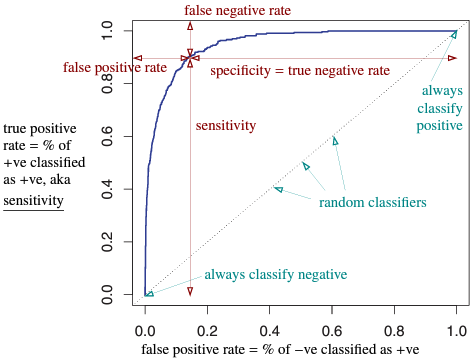
\includegraphics[scale=0.5]{./images/ROC-curve.png}
    \ruler%TODO Remove

    \section{Polynomial Regression (Lecture 11)}
    Replace each $x_i$ with feature vector $\Phi(x_i)$ with all terms of degree $p$ polynomial.
    e.g.,$ \Phi(x_i) = \begin{bmatrix} x^2_{i1} & x_{i1}x_{i2} & x^2_{i2} & x_{i1} & x_{i2} &  1 \end{bmatrix}^\top$
    \ruler%
    Log. Reg. + quadratic features = same form of posteriors as QDA\@.

    \section{Statistical Justification For Regression (Lecture 12)}
    Typical model of reality:
    $\forall X_i, \, y_i = g(X_i) + \epsilon_i\,\,$: $\epsilon_i \sim D^\prime$ where $D^\prime$ has mean 0.

    Ideal approach: choose $h(X_i) = \E_y[Y | X = X_i] = g(X_i) + \E[\epsilon_i] = g(X_i)$
    \subsection{Least Squares Cost Function From MLE}
    Suppose $\epsilon_i \sim \Norm\left(0, \sigma^2\right) \implies y_i \sim \Norm\left(g(\va{x}_i), \sigma^2\right)$. We're going to try to estimate $g(\va{x})$, which is defined by some weights $\va{w}$. The probability of $y_i$, given it's parameters for its distribution, is a pdf $f(y_i)$ \& the log likelihood is:
    \begin{align*}
        \ell(g; \bX, \va{y}) & = \ln(\prod_{i=1}^n f(y_i))
        = \sum_{i = 1}^{n} \ln(f(y_i))
        = -\frac{1}{2\sigma^2}\sum_{i = 1}^{n}\left(y_i - g(\va{x}_i)\right)^2 - C
    \end{align*}
    Maximumizing this is equivalent to minimizing $\sum_{i = 1}^{n}\left(y_i - g(\va{x}_i)\right)^2 = \text{RSS}$

    \subsection{Logistic Loss from MLE}
    Consider $P[\va{x}_i \in \text{class C}] = y_i$ as the actual probability, with $h(\va{x}_i)$ as the predicted probability. For $\beta$ hypothetical repetitions, where $y_i\beta$ samples belong to class C and $(1 - y_i)\beta$ do not. The likelihood of $h$ given the data is:
    \[
        \mathscr{L}(h; \bX, \va{y}) = \prod_{i = 1}^{n} h(\va{x}_i)^{y_i \beta} (1 - h(\va{x}_i))^{(1 - y_i)\beta}
    \]
    \[
        \ell(h; \bX, \va{y}) = \beta \sum_{i = 1}^{n} \left[ y_i \ln (h(\va{x}_i)) + (1 - y_i) \ln (1 - h(\va{x}_i)) \right]
    \]
    Maximizing the log likelihood $\ell(h)$ is equivalent to minimizing logistic losses.

    \subsection{The Bias-Variance Decomposition}
    There are 2 sources of error in a hypothesis $h$:
    \begin{itemize}
        \item \textbf{bias}: error due to inability of hypothesis $h$ to fit $g$ perfectly.
        \item \textbf{variance}: error due to fitting random noise in data, e.g., we fit linear $g$ with a linear $h$, yet $h \neq g$.
    \end{itemize}

    Model: $X_i \sim D$, $\epsilon_i \sim D^\prime$ and $y_i = g(X_i) + \epsilon_i$. Fit hypothesis $h$ to $\bX, \va{y}$. Now $h$ is a r.v., because of the random noise $\epsilon$. Let $z$ be an arbitrary pt and $\gamma = g(z) + \epsilon$
    Now the risk fn when loss is the squared errror is:\\
    $R(h) = \E[L(h(z), \gamma)] \leftarrowtail$ exp over possible training set $X, y$ and values of $\gamma$\\
    $R(h) = \E[(h(z) - \gamma)^2]$\\
    $R(h) = \E[h(z)^2] + \E[\gamma^2] - 2\E[\gamma h(z)]$\\
    $R(h) = \Var(h(z)) + {\E[h(z)]}^2 + \Var(\gamma) + {\E[\gamma]}^2 - 2\E[\gamma] \E[h(z)]$\\
    $R(h) = \left(\E[h(z)] - \E[\gamma]\right)^2 + \Var(h(z)) + \Var(\gamma)$\\
    $R(h) = \underbrace{\left(\E[h(z)] - \E[\gamma]\right)^2}_{\text{bias}^2 \text{ of method}} + \underbrace{\Var(h(z))}_{\text{variance of method}} + \underbrace{\Var(\epsilon)}_{\text{irreducible error}}$\\
    \begin{itemize}[label=$\bullet$]
        \item \textbf{Underfitting}: Too much bias
        \item \textbf{Overfitting}: Too much variance
        \item Training Error reflects bias but not variance
        \item Test error reflects both.
    \end{itemize}

    \section{Linear Regression Regularization (Lecture 13)}
    \textbf{Trading off bias/variance}: some increase in bias can give big decrease in var.
    \ruler%
    \textbf{Ridge regression} is like $L2$ regularization: \\
    $\hat{\va{w}} = \text{arg }\min_{\va{w}}\norm{\va{y} - \bX\va{w}}^2 + \lambda \norm{\va{w}}^2$, for some cost function $J$ on classifier $h$\\
    Minimized w/ Calculus\\
    $\hat{\va{w}}^{\text{ridge}}=\inv{(\bX^{\top}\bX+\lambda\bI)}\mat{X}^{\top}\va{y}$
    \ruler%
    \textbf{Lasso regression} is like $L1$ regularization:\\

    Minimized w/ Calculus (it's also a quadratic program)\\
    While ridge regression leads to reduced, but rare non-zero values of the weights,
    Lasso regression forces some weights to be zero.
    \ruler%
    \textbf{Bayesian analysis}:
    Ridge regression is equivalent to a MAP estimate with a gaussian prior.
    Lasso regression is equivalent to a MAP estimate with a Laplace prior.
    % --------------------------------
    \section*{Misc}
    \begin{itemize}
        \item \textbf{Centering} $\bX$: This involves subtracting $\bm{\mu}^T$ from each row of $\bX$. Symbolically, $\bX$ transforms into $\bar{\bX}$.
        \item \textbf{Decorrelating} $\bX$: This process applies a rotation $\mat{Z} = \bar{\bX}\mathbf{V}$, where $\text{Var}(\mathbf{R}) = \mathbf{V\Lambda V}^T$. This step rotates the sample points to the eigenvector coordinate system.
        \item \textbf{Sphering:}  $\bar{\bX}$: applying transform $\mat{W} = \bar{\bX} \text{Var}(\mathbf{R})^{-\frac{1}{2}}$
        \item \textbf{whitening} \(\bX\): centering + sphering, \(\bX \rightarrow \mat{W}\)
    \end{itemize}


    \section{Decision Trees (Lecture 14, 15)}
    Nonlinear method for classification or regression. Cuts x-space into rectangular cells. Works well with both categorial and quantiative features. They're fast, interpretable, robost to irrelevant features, but not best at prediction $\rightarrow$ high variance often mitigated by ensemble learning.

    \textbf{For classification} the learning algorithm is a greedy, top-down learning heuristic. Let $S$ be subset of sample point indices:\\
    \begin{algorithmic}
        \Function{GrowTree}{$S$}
        \If{all $y_i = C$ for all $i \in S$ and some class $C$}
        \State \Return \textit{new} leaf($C$)
        \Else
        \State Choose best splitting feature $k$ and splitting value $\beta$
        \State $S_L = \{ i \in S: \mat{X}_{ik} < \beta \}$
        \State $S_R = \{ i \in S: \mat{X}_{ik} \ge \beta \}$
        \State \Return \textit{new} node$\big(k$, $\beta$, \Call{GrowTree}{$S_L$}, \Call{GrowTree}{$S_R$}$\big)$
        \EndIf
        \EndFunction
    \end{algorithmic}
    \textbf{Optimal Split Selection:}
    Evaluate all possible $(k, \beta)$ splits and choose the one that minimizes the weighted impurity cost:
    \[
        J(S, k, \beta) = \frac{|S_L| J(S_L) + |S_R| J(S_R)}{|S_L| + |S_R|}
    \]
    where entropy $J(S) = -\sum_{c} p_c \log_2(p_c)$ , $\quad\text{with } p_c = \frac{|\{ i \in S : y_i = c \}|}{|S|}$

    \textbf{Information Gain,} defined as $IG(S, k, \beta) = J(S) - J(S, k, \beta)$\\
    IG maximization is equivalent to entropy minimization post-split.\\

    \textbf{Pruning}: Grow tree too large; greedily remove each split whose removal improves validation performance on test data that lies on these splits.\\
    \textbf{For regression: } Leafs stores mean response for training pts in that region. Different cost function: $J(S) = RSS = \frac{1}{|S|} \sum_{i \in S}^{} (y_i - \mu_s)^2 = \Var\left(\{y_i : i \in S\}\right)$
    \textbf{Ensemble Methods}
    Decision trees often suffer from high variance, which can lead to overfitting. Ensemble methods, by combining multiple trees, aim to reduce this variance and improve predictive performance.

    \textbf{Bagging}: Given n-point training samples, generate random subsamples of size $n'$ by sampling \underline{\textit{with replacement}}. If $n' = n \rightarrow \sim 63.2\%$ are chosen. Idea: Points chosen $j$ times have greater weight in cost when misclassified.
    \textbf{Random Forest}: Enhance Bagging by reducing correlation between different trees with feature randomness at each split. This process ensures that the ensemble does not rely too heavily on any single feature and makes trees within the forest less identical.


    \columnbreak
    \section{Kernels (Lecture 16)}
    In many learning algorithms, the weights can be written as a linear combo of training points, that is, $\va{w} = \bX^\top \va{\alpha} = \sum_{i = 1}^{n} \alpha_i \va{x_i}$, for some $\va{\alpha} \in \R^n$.

    We can subsitute this identity into alg, and optimize $n$ \underline{dual weights} $\alpha$ instead of the $\va{w}$ of the primal problem.
    \textbf{Kernel Trick:} Enables learning algorithms to operate in high-dimensional space without explicitly computing the transformations.

    \textbf{Kernel Ride Regression}
    \begin{itemize}
        \item Transform the training set $X$ using a kernel function $k(x, z)$, creating a kernel matrix $K$.
        \item Solve $(K + \lambda I)a = y$ for the dual coefficients $a$, where $\lambda$ is the regularization parameter.
        \item Predictions for a new point $z$ are made by $h(z) = \sum_{i=1}^{n} a_i k(x_i, z)$.
    \end{itemize}
    ---
    \begin{itemize}
        \item Center $\bX$: $\va{x_i} \leftarrow \va{x}_i - \mu_x$, except ficticious dimension, $\va{x}_{i, d + 1} = 1$
        \item Center $\va{y}$: $\va{y} \leftarrow \va{y} - \mu_y$.
    \end{itemize}
    In ridge regression, recall the normal equations:
    \[
        \left(\bX^\top \bX + \lambda \mat{I}'\right) \va{w} = \bX^\top \va{y}
    \]
    Where $I'$ is the identity matrix with 0 at the position of the ficticious dimension so that we don't penalize the bias. In order for the condition that the weights be a linear combination of training points to be satisfied, we need to penalize the bias.

    Now the objective function is: (subsiting $\va{w} = \bX^\top \va{\alpha}$)
    \[
        \norm{\bX^\top \left(\bX \va{\alpha}\right) - \va{y}}^2 + \lambda \norm{\bX^\top \va{\alpha}}^2
    \]
    \begin{itemize}
        \item \textbf{Training}: Solve $\left(\bX\bX^\top + \lambda \mat{I}\right) \va{\alpha} = \va{y}$, for $\va{\alpha}.$
        \item \textbf{Testing}: Regression fn is $h(\va{z}) = \va{w}^\top \va{z} = \va{\alpha}^\top \bX \va{z} = \sum_{i = 1}^{n} \alpha_i (\va{x}_i^\top \va{z})$
    \end{itemize}
    Let $k(\va{x}, \va{z}) = \va{x}^\top \va{z}$ be the kernel function. \\
    Let $\mat{K} = \bX \bX^\top \in \R^{n \times n}$ be the kernel matrix with $\mat{K}_{ij} = k(\va{x}_i, \va{x}_j)$. \\
    \textbf{Kernel Ridge Regr. Alg:}
    \begin{algorithmic}
        \State Initialize the kernel matrix $\mat{K}$ \Comment{$\O(n^2d)$ time}
        \State Solve $(\mat{K} + \lambda \mat{I}) \va{\alpha} = \va{y}$ \Comment{$\O(n^3)$ time}
        \For{each test point $z$, compute}
        \State $h(z) = \sum_{i = 1}^{n} \alpha_i k(\va{x}_i, z)$ \Comment{$\O(nd)$ time per test pt  }
        \EndFor
    \end{algorithmic}
    \subsection{The Kernel Trick (aka Kernelization)}
    \textbf{Polynomial kernel} of degree $p$ is $k(\va{x}, \va{z}) = (\va{x}^\top \va{z} + 1)^p$\\
    \textbf{Theorm}: $(\va{x}^\top \va{z} + 1)^p = \Phi^T(\va{x}) \Phi(\va{z})$ for some feature map $\Phi$\\
    \textit{Note} now we can compute $\Phi^T(\va{x}) \Phi(\va{z})$ in $\O(d)$ time instead of $\O(d^p)$

    \textbf{Gaussian (RBF) Kernel:} $k(x, z) = \exp\left(-\frac{\|x - z\|^2}{2\sigma^2}\right)$, measures the similarity, or closeness, of $x$ and $z$ with a parameter $\sigma$ controlling the width of the Gaussian.

    \textbf{Choosing $\sigma$ in Gaussian Kernels:}
    \begin{itemize}
        \item Trade-off between bias and variance: larger $\sigma$ leads to smoother models with higher bias and lower variance.
        \item Selected based on validation performance, optimizing for generalization.
    \end{itemize}


    % ########################
    % ### Neural Networks ####
    % ########################
    \section{Neural Networks (Lecture 17)}
    Input Layer: $x_1, \dots, x_d : x_{d + 1} = 1$\\
    Hidden Units: $h_1, \dots, h_m: h_{m + 1} = 1$\\
    Output Layer: $z_1, \dots, z_k$

    Layer 1 weights $V \in \R^{m \times (d + 1)}$ (row $i$, $V_i^\top$ contains all the weights from previous layer, coming into hidden unit $i$)\\
    Layer 2 weights $W \in \R^{k \times (m + 1)}$\\

    $\va{z} = \va{s}(\mat{W} \va{h}) = \va{s}(\mat{W} \va{s}_1(\mat{V} \va{x})) \quad$
    where $\va{s}_1$ is the activation function applied element wise to vector, with last component set to 1.

    \textbf{Acitvation Functions}:
    \begin{itemize}
        \item $s(\gamma) = \sigma(\gamma) = \frac{1}{1 + e^{-\gamma}} \implies \sigma^\prime(\gamma) = \sigma(\gamma)(1 - \sigma(\gamma))$
        \item $s(\gamma) = \sigma_\text{ReLU}(\gamma) = \max(0, \gamma) \implies \sigma_\text{ReLU}^\prime(\gamma) = \begin{cases} 1 & \gamma > 0 \\ 0 & \gamma \leq 0 \end{cases}$
    \end{itemize}

    \begin{figure}[H]
        \centering
        \includegraphics[width=\columnwidth]{images/backprop.png}
    \end{figure}
    \begin{figure}[H]
        \centering
        \includegraphics[width=\columnwidth]{images/backprop22.png}
    \end{figure}
    \begin{figure}[H]
        \centering
        \includegraphics[width=\columnwidth]{images/backprop4.png}
    \end{figure}


    % ########################
    % ######## PCA ###########
    % ########################
    \section{PCA: Principal Component Analysis (Lecture 20)}
    \textbf{Goal:} Identify \( k \) principal directions to maximize variance capture after projecting data onto these components, enhancing computational efficiency and reducing overfitting by eliminating irrelevant features.


    \textbf{Assumptions:} Assume \( \mathbf{X} \) is centered, i.e., \( \sum_{i=1}^n \mathbf{x}_i = 0 \).

    \textbf{Orthogonal Projection} of a point \( \mathbf{x} \) onto a vector \( \mathbf{w} \) is given by:
    \[
        \tilde{\mathbf{x}} = \frac{\mathbf{x} \cdot \mathbf{w}}{\|\mathbf{w}\|^2} \mathbf{w}
    \]
    Aim: Find the best \( \mathbf{w} \) that captures the maximum variance after projecting.

    \textbf{Principal Coordinates and Components:}
    Given orthonormal directions \( \mathbf{v}_1, \ldots, \mathbf{v}_k \), the \underline{\textit{projection}} of \( \mathbf{x} \) onto these vectors is:
    \[
        \tilde{\mathbf{x}} = \sum_{i=1}^k (\mathbf{x} \cdot \mathbf{v}_i) \mathbf{v}_i
    \]
    where \( \mathbf{x} \cdot \mathbf{v}_i \) are the \underline{\textit{principal coordinates}}. The \underline{\textit{principal components}} are unit eigenvectors \( \mathbf{v}_1, \ldots, \mathbf{v}_d \) of the covariance matrix \( \hat{\Sigma} = \frac{1}{n} \mathbf{X}^\top \mathbf{X} \), associated with its eigenvalues \( \lambda_1 \leq \lambda_2 \leq \cdots \leq \lambda_d \).

    \begin{algorithmic}
        \Function{PCA Algorithm}{$\mat{X}$, $\mat{X}_\text{test}$}
        \State Center \( \mathbf{X} \)
        \State Compute unit eigenvectors and eigenvalues of \( \mathbf{X}^\top \mathbf{X} \)
        \State Choose \( k \) (optionally based on the size of eigenvalues)
        \State Select the top \( k \) eigenvectors \( \mathbf{v}_{d-k+1}, \ldots, \mathbf{v}_d \) for the best \( k \)-dimensional subspace
        \State Compute the \( k \) principal coordinates \( \mathbf{x} \cdot \mathbf{v}_i \) for each training/test point
        \EndFunction
    \end{algorithmic}

    \textbf{Derivation 2: Variance Maximization:} Find $\bw$ that maximizes
    $$\Var(\{\tilde{\bx}_1, \tilde{\bx}_2, \dots, \tilde{\bx}_n\}) = \frac{1}{n} \frac{\norm{\bX \bw}^2}{\norm{\bw}^2} = \frac{1}{n} \frac{\bw^\top \bX^\top \bX \bw}{\bw^\top\bw} = \frac{1}{n}\text{Raylegh Quotient}(\bX^\top \bX)$$

    \hspace*{3pt}\textbf{Theorm}: $\va{v}_d$ maximizes this variances.

    \textbf{Derivation 3: Projection Distance Minimization}:\\
    Find direction $\bw$ that minimizes the mean of squared projection distance.

    $$
        \sum_{i = 1}^{n}\norm{\bx_i - \tilde{\bx}_i}^2 = \sum_{i = 1}^{n} \norm{\bx_i - \frac{\bx_i \cdot \bw}{\norm{\bw}^2} \bw}^2
    $$
    $$
        = \sum_{i = 1}^{n} \left(\norm{\bx_i}^2 - \left(\bx_i \cdot \frac{\bw}{\norm{\bw}}\right)^2\right) = C - n(\text{variation from derivation 2})
    $$
    Minimizing mean squared project distance $\equiv$ Maximizing variance.

    % ###############################################
    % ####### SVD and Clustering (Lecture 21) #######
    % ###############################################
    \section{SVD, Clustering (Lecture 21)}
    \textbf{SVD}:
    Problem with PCA is that computing $X^\top X$ is expensive, taking $\O(nd^2)$.
    \[
        \left[\mat{X}\right]_{n \times d} = \left[\mat{U}\right]_{n \times d} \left[\mat{D}\right]_{d \times d} \left[\mat{V}\right]_{d \times d}^T = \sum_{i = 1}^{d} \delta_i \va{u}_i \va{v}^T_i \quad \text{ when } n \ge d
    \]
    \begin{itemize}[label=\textbullet]
        \item The number of non-negative singular values corresponds to the rank of $\mat{X}$.
        \item $\va{v}_i$ is an eigenvector of $\mat{X}^T X$ with eigenvalue $\delta_i^2$.
        \item We can find the $k$ greatest singular values \& corresp vectors in $\O(ndk)$
        \item Row $i$ of $\mat{U}\mat{D}$ gives the principle coordinates of sample $\mat{X}_i$
    \end{itemize}
    \ruler%
    \textbf{Clustering}: Partition data into $K$ clusters so pts in a cluster are more similar than across clusters.

    \textbf{K-Means Clustering} goal is to parition pts into $k$ disjoint clusters to minimize the sum of squared distances from each point to its cluster center.
    \[
        \boxed{\text{Find } \va{y} \text{ that minimizes} \sum_{i = 1}^{k} \sum_{y_j = i} \norm{\mat{X}_j - \va{\mu}_i}^2}
    \]
    Where, $\va{\mu}_i = \frac{1}{n_i} \sum_{y_j = i} \mat{X}_j$ is the mean of cluster $i$, given $n_i$ pts in cluster $i$.
    Problem is NP-hard, $\O(nk^n)$. Use heuristic, alternating between 2 steps.
    \begin{enumerate}
        \item Fixing labels $y_j$ and updating cluster means $\mu_i$ to min the obj\@. fn.
        \item Fixing $\va{\mu}_i$ and updating labels $y_j$ to minimize the objective function.
    \end{enumerate}
    Repeats until no assignments change. Both steps decrease obj\@. fn, \textit{unless} they change nothing. Hence alg\@. must terminate. We can show through calculus:
    \begin{enumerate}
        \item The optimal $\va{\mu}_i$ is the mean of its cluster
        \item The optimal $\va{y}$ assigns each pt $\mat{X}_j$ to nearest center $\va{\mu}_i$
    \end{enumerate}
    \textbf{Initalization Stratigies}
    \begin{itemize}
        \item \textbf{Forgy Method}: Choose $k$ random sample pts to be inital $\va{\mu}_i$'s; go to step 2.
        \item \textbf{Random Parition}: randmly assign each sample pt to a cluster; go to step 1.
        \item \textbf{K-Means++}: Like Forgy, but biased distribution, choosing centers far apart.
    \end{itemize}
    Equivalent Object Function: called \underline{\textit{The Within-Cluster Variation}}: (no $\va{\mu}_i$)
    $
        \min_{\va{y}} \sum_{i = 1}^{k} \frac{1}{n_i} \sum_{y_j = i} \sum_{y_m = i} \norm{\mat{X}_j - \mat{X}_m}^2.
    $
    Minimum is twice the  prev\@. obj\@. fn\@.
    \ruler%
    \textbf{Hierarchical Clust}: Builds tree of clusters; every subtree is cluster. Built using
    \begin{itemize}[label=\textbullet]
        \item \textbf{Agglomerative (Bottom-up)}: Start with each point as a cluster, then merge the closest pairs until one cluster remains.
        \item \textbf{Divisive (Top-down)}: Start with all points in one cluster, then iteratively split the most diverse cluster.
    \end{itemize}
    We need a distance fn for clusters $A, B$. Here are 4 common ones :
    \begin{itemize}
        \item \textbf{Complete Linkage}: Max distance between any points in two clusters.
        \item \textbf{Single Linkage}: Min distance between any points in two clusters.
        \item \textbf{Average}: Avg dist between all points in clusters. $d(A, B) = \frac{1}{|A| |B|} \sum_{w \in A}^{} \sum_{x \in B}^{} d(w, x)$
        \item \textbf{Centroid Linkage}: dist between centroids of clusters. $d(A, B) = d(\mu_A, \mu_B)$
    \end{itemize}
    Greedy Agglomerative Alg: repeatedly \textit{fuse} the 2 clusters that minimize $d(A, B)$. Naive takes $\O(n^3)$, done in $\O(n^2)$ for complete and single linkage\\
    \textbf{Dendrogram}: Illustration of the cluster hierarchy. Vertical axis encodes all the linkage distances. Horizontal axis has no meaning.
    The complete linkage tends to give balanced trees.

    % ##############################
    % ####### LEARNING THEORY ######
    % ##############################
    \section{Learning Theory (Lecture 23)}
    Learning theory explores how machine learning algs generalize from training data to unseen data. It involves understanding the constraints needed for a learner to make predictions on new data effectively.

    \textbf{Range Space}: Defined by $(P, H)$ where $\bm{P}$ is the set of all train/test points and $\bm{H}$ is the hypothesis class or a set of classifiers. Each hypothesis $h \in H$ identifies which points are predicted to be in a particular class.

    \textbf{Risk and Empirical Risk}:
    \underline{\textit{Risk (Generalization Error) $R(h)$}:} The prob\@. that a hypothesis $h$ misclassifies a randomly drawn point from distribution $\mathcal{D}$.
    \underline{\textit{Empirical Risk $\hat{R}(h)$}:} The proportion of training data misclassified by $h$, which better approximates $R(h)$ as the size of the training set increases.

    \textbf{Hoeffding's Inequality}:
    Tells us probability of bad Risk estimate.
    \[
        \Pr(|\hat{R}(h) - R(h)| > \epsilon) \leq 2e^{-2\epsilon^2n},
    \]
    where $\epsilon$ is the error margin and $n$ is \# of samples. This shows that larger $n$ expoenntially decays the chance of deviation between $\hat{R}(h)$ and $R(h)$.

    \textbf{Empirical Risk Minimization (ERM)}:
    Selects the hypothesis $\hat{h}$ that minimizes $\hat{R}(\hat{h})$ among $H$. ERM is infeasible to pick optimal hypothesis.

    \textbf{Dichotomies and Sample Complexity}:
    A dichotomy created by a hypothesis $h$ over set $X$ categorizes points into class $C$ or its complement. The number of possible dichotomies, $\Pi$, influences the likelihood of misleadingly low empirical risks. If $H$ induces $\Pi$ dichotomies, then:
    \[
        \Pr(\text{at least one dichotomoy has }|\hat{R} - R| > \epsilon) \le \delta = 2\Pi e^{-2\epsilon^2 n}
    \]
    with confidence $1 - \delta$, $\forall h \in H$, $|\hat{R}(h) - R(h)| \le \epsilon = \sqrt{\frac{1}{2n} \ln \frac{2\Pi}{\delta}}$. This formulation reveals that increasing $n$ and reducing $\Pi$ enhances risk estimates' reliability.

    \textbf{Optimal Risk Approximation}:
    If $h^* \in H$ minimizes $R(h^*)$, then with high probability $1 - \delta$, the selected hypothesis $\hat{h}$ that minimizes $\hat{R}(\hat{h})$ fulfills:
    \[
        R(\hat{h}) \le \hat{R}(\hat{h}) + \epsilon \le \hat{R}(h^*) \le R(h^*) + 2\epsilon
    \]

    \textbf{Sample Complexity}:
    The minimum \# of samples required to ensure that $\epsilon$ approximation accuracy with confidence $1 - \delta$ is:
    \[
        n \ge \frac{1}{2\epsilon^2} \ln \frac{2\Pi}{\delta}
    \]







    % ########################
    % ####### ADA BOOST ######
    % ########################
    \section*{AdaBoost: Adaptive Boosting (Lecture 24)}
    An ensemble method for classification (or regression) that trains $T$ learners on \underline{weighted} samples points, gives bigger votes to more accurate learners, and increases weights of misclassified points (pay more attention to this point), with the goal of \textit{\underline{reducing bias}}. If every learner has $\text{err} < 0.5$, $M(\va{x})$ training $\text{err} \rightarrow 0$ as $T \rightarrow \infty$.

    \textbf{Input}: $\mat{X} \in \R^{n \times d}$ and $\va{y} \in \R^n$ with $y_i = \pm 1$ (not natural fit if labels arent bin).
    \textbf{Idea}:
    \begin{itemize}
        \item \textbf{Training Classifiers:} Sequentially train $T$ classifiers $G_1, \dots, G_T$
        \item \textbf{Weight Adjustment:} Weight for training pt $\va{x}_i$ in iteration $t$ for $G_t$ grows accoring to how many of $G_1, \dots, G_{t - 1}$ misclassified it.
        \item \textbf{Meta Learner:} is a linear combobination of all $T$ classifiers. Output is not binary; apply the sign function for binary classification.
    \end{itemize}
    \ruler%
    \textbf{Risk Minimization:} Risk of the meta learner is average exponential loss $L(\rho, \ell) = e^{-\rho \ell}$, and minimize it to adjust $\beta_T$ and select the optimal classifier $G_T$ for each round:

    \begin{align*}
        n * \text{Risk} & = \sum_{i = 1}^{n} L(M(\va{x}_i), y_i)=\sum_{i = 1}^{n} \prod_{t = 1}^{T} \exp(-y_i \beta_t G_t(\va{x}_i))                         \\
                        & = \sum_{i = 1}^{n} w^{(T)}_i \exp(-y_i \beta_T G_T(\va{x}_i))                                                                      \\
                        & = e^{-\beta_T} \sum_{y_i = G_T(\va{x}_i)} w^{(T)}_i + e^{\beta_T}\sum_{y_i \neq G_T(\va{x}_i)} w^{(T)}_i                           \\
                        & = \cancel{e^{-\beta_T} \sum_{i = 1}^{n} w^{(T)}_i} + \cancel{(e^{\beta_T} - e^{-\beta_T})} \sum_{y_i \neq G_T(\va{x}_i)} w^{(T)}_i
    \end{align*}
    where \( w^{(T)}_i = \prod_{t = 1}^{T - 1} \exp(-y_i \beta_t G_t(\va{x}_i)) \) is the cumulative weight adjusted for each sample up to classifier \( T-1 \).
    Therefore, the optimal classifier $G_T$ minimizes the sum of weights of misclassified points.

    \textbf{Recursive Weight Update:}
    To focus training on misclassified points:
    \[
        w^{(T+1)}_i = w^{(T)}_i \exp(-y_i \beta_T G_T(\va{x}_i)) =
        \begin{cases}
            w^{(T)}_i \exp(-\beta_T) & \text{if } y_i = G_T(\va{x}_i)    \\
            w^{(T)}_i \exp(\beta_T)  & \text{if } y_i \neq G_T(\va{x}_i)
        \end{cases}
    \]

    \textbf{Optimization for $\beta_T$:} Solve for $\beta_T$ by setting the derivative of the risk with respect to $\beta_T$ equal to zero, deriving that:
    \[
        \beta_T = \frac{1}{2} \ln\left(\frac{1 - \text{err}_T}{\text{err}_T}\right),
    \]
    where $\text{err}_T$ is the weighted proportion of misclassified instances by $G_T$. Therefore a perfect learner ($\text{err}_T = 0$) has $\beta_T = \infty$
    \ruler%
    \begin{algorithmic}
        \Function{AdaBoost}{$\mat{X}$, $\va{y}$}
        \State Initialize weights $w_i = \frac{1}{n}$ for all $i$
        \For{$t \leftarrow 1$ to $T$}
        \State Train classifier $G_t$ on $(\mat{X}, \va{y})$, using weights $\va{w}$
        \State Calculate error $\text{err}_t$
        \State Calculate $\beta_t$ using $\text{err}_t$
        \State Update weights: $w_i \leftarrow w_i \exp(- y_i \beta_t G_t(x_i))$
        \EndFor
        Return metalearner $h(\va{z}) = \text{sign}(\sum_{t = 1}^{T} \beta_)$
        \EndFunction
    \end{algorithmic}

    \section{K-Nearest Neighbor (Lecture 25)}
    \textbf{Idea}: Given query point $\va{q}$, find the $k$ training pts nearest to $\va{q}$.\\
    \textbf{Theorem}: as $n \rightarrow \infty$, the 1-NN error rate is $< 2B-B^2$ where $B = $ bayes risk.
    \textbf{Theorem}: As $n \rightarrow \infty$, $k \rightarrow \infty$, and $\frac{k}{n}\rightarrow 0$ ($n$ grows faster than $k$), k-NN error rate converges to $B$

    \textbf{Exhaustive k-NN: Algorithm}:\\
    Given query point $q$:
    \begin{itemize}[label=\textbullet]
        \item Scan through all $n$ training pts, computing (squared) distances to q.
        \item Maintain a max-heap with the $k$ closest training points seen so far.
        \item Time to train classifier: $\O(0)$ (no time)
        \item Query Time: $\O(nd + n\log k)$, expected $\O(nd + k\log(n) \log(k))$ if random point order.
    \end{itemize}

    \textbf{Voronai Diagrams}:\\
    Let $X$ be a point set. the \underline{Voronoi cell} of $w \in X$ is $\text{Vor } w = \big\{p \in \R^d : \norm{p - w} \leq \norm{p - v} \; \forall v \in X\big\}$\\
    The \textit{Voronoi diagram} of $X$ is the set of $X$'s Voronoi cells.

    \section{K-Nearest Neighbor (Lecture 25)}
    \textbf{Principle}: For a query point $\va{q}$, classify based on the majority label among its $k$ nearest training points.

    \textbf{Theorem}: Under certain conditions:
    \begin{itemize}[label=\textbullet]
        \item For 1-NN, as $n \rightarrow \infty$, the error rate is less than twice the Bayes risk $B$.
        \item For k-NN, as $n \rightarrow \infty$, $k \rightarrow \infty$, and $\frac{k}{n} \rightarrow 0$, the error rate converges to $B$.
    \end{itemize}

    \textbf{Exhaustive k-NN Algorithm}:
    \begin{itemize}[label=\textbullet]
        \item Compute squared distances from $\va{q}$ to all $n$ training points.
        \item Use a max-heap to maintain the $k$ closest points.
        \item \textit{Complexity}: Training: $\O(0)$, Query: $\O(nd + n\log k)$.
    \end{itemize}

    \textbf{Voronoi Diagrams}:
    \begin{itemize}[label=\textbullet]
        \item The Voronoi cell for a point $w \in X$ is defined as: $\text{Vor}(w) = \{ p \in \R^d : \|p - w\| \leq \|p - v\|, \forall v \in X \}$.
        \item Used for 1-NN to locate the nearest training point to a query point.
        \item \textit{Complexity}: For low dimensions ($2-5$), efficient; for higher, consider k-d trees.
    \end{itemize}

    \textbf{k-d Trees}:
    \begin{itemize}[label=\textbullet]
        \item Space-partitioning data structure to organize points in k-dimensional space.
        \item Splits along axis-aligned hyperplanes for efficient nearest neighbor search.
        \item \textit{Building}: $\O(nd \log n)$, \textit{Query}: sublinear, depends on dimensionality.
    \end{itemize}

    \textbf{Key Advantages}:
    \begin{itemize}[label=\textbullet]
        \item Non-parametric and simple.
        \item Effective for small datasets and low dimensionality.
    \end{itemize}

    \textbf{Challenges}:
    \begin{itemize}[label=\textbullet]
        \item High query time in large datasets.
        \item Curse of dimensionality: performance degrades as dimensionality increases.
    \end{itemize}




\end{multicols*}
\end{document}
